\documentclass{article}
\usepackage[utf8]{inputenc}
\documentclass[UTF8]{ctexart}
\usepackage[version=4]{mhchem}
\usepackage{float}

\title{Brief Exploration of How the Difference of Dipole Moment between 127 isomers of \ce{C6H6} Changes their Total Energy and the Highest Occupied Molecular Orbitals Energy (HOMOE) }
\author{James Chen \\ \ Instructor: Prof. Sun, Dr. Hu}
\date{January 2021}

\usepackage{natbib}
\usepackage{graphicx}

\begin{document}

\maketitle

\section{Introduction}
In the history of chemistry, many scientists had made their own assumption of the molecular structure of \ce{C6H6}, and the experiments finally proved that the Benzene is the most stable structure of \ce{C6H6}. With the development of computer simulation technology, we can now do Geometry Optimization simulations for all the isomers of \ce{C6H6} and try to find out which key factor of the molecular might influence the stability. In this experiment, we decided to explore how the difference of dipole moment between isomers of \ce{C6H6} changes their Total Energy and the Highest Occupied Molecular Orbitals Energy (HOMOE) \\ With simple compute of the degree of unsaturation of \ce{C6H6}, we can determine that there are 127 isomers of \ce{C6H6} (not including chiral isomers and stereoisomerism)



\section{Overview}
For all 127 Geometry Optimization simulations, 18 failed, so the success rate of the Geometry Optimization simulations is 85.82\%, which is higher than what I anticipated. 


\section{Dipole Moment with Total Energy}
As we can see from the graph that the dipole moment of each isomer and the molecule's total energy is not so relevant as I thought. But we can see the total energy concentrated at a certain area that ranges from 232.15 to 232.00.
\begin{figure}[H]
\centering
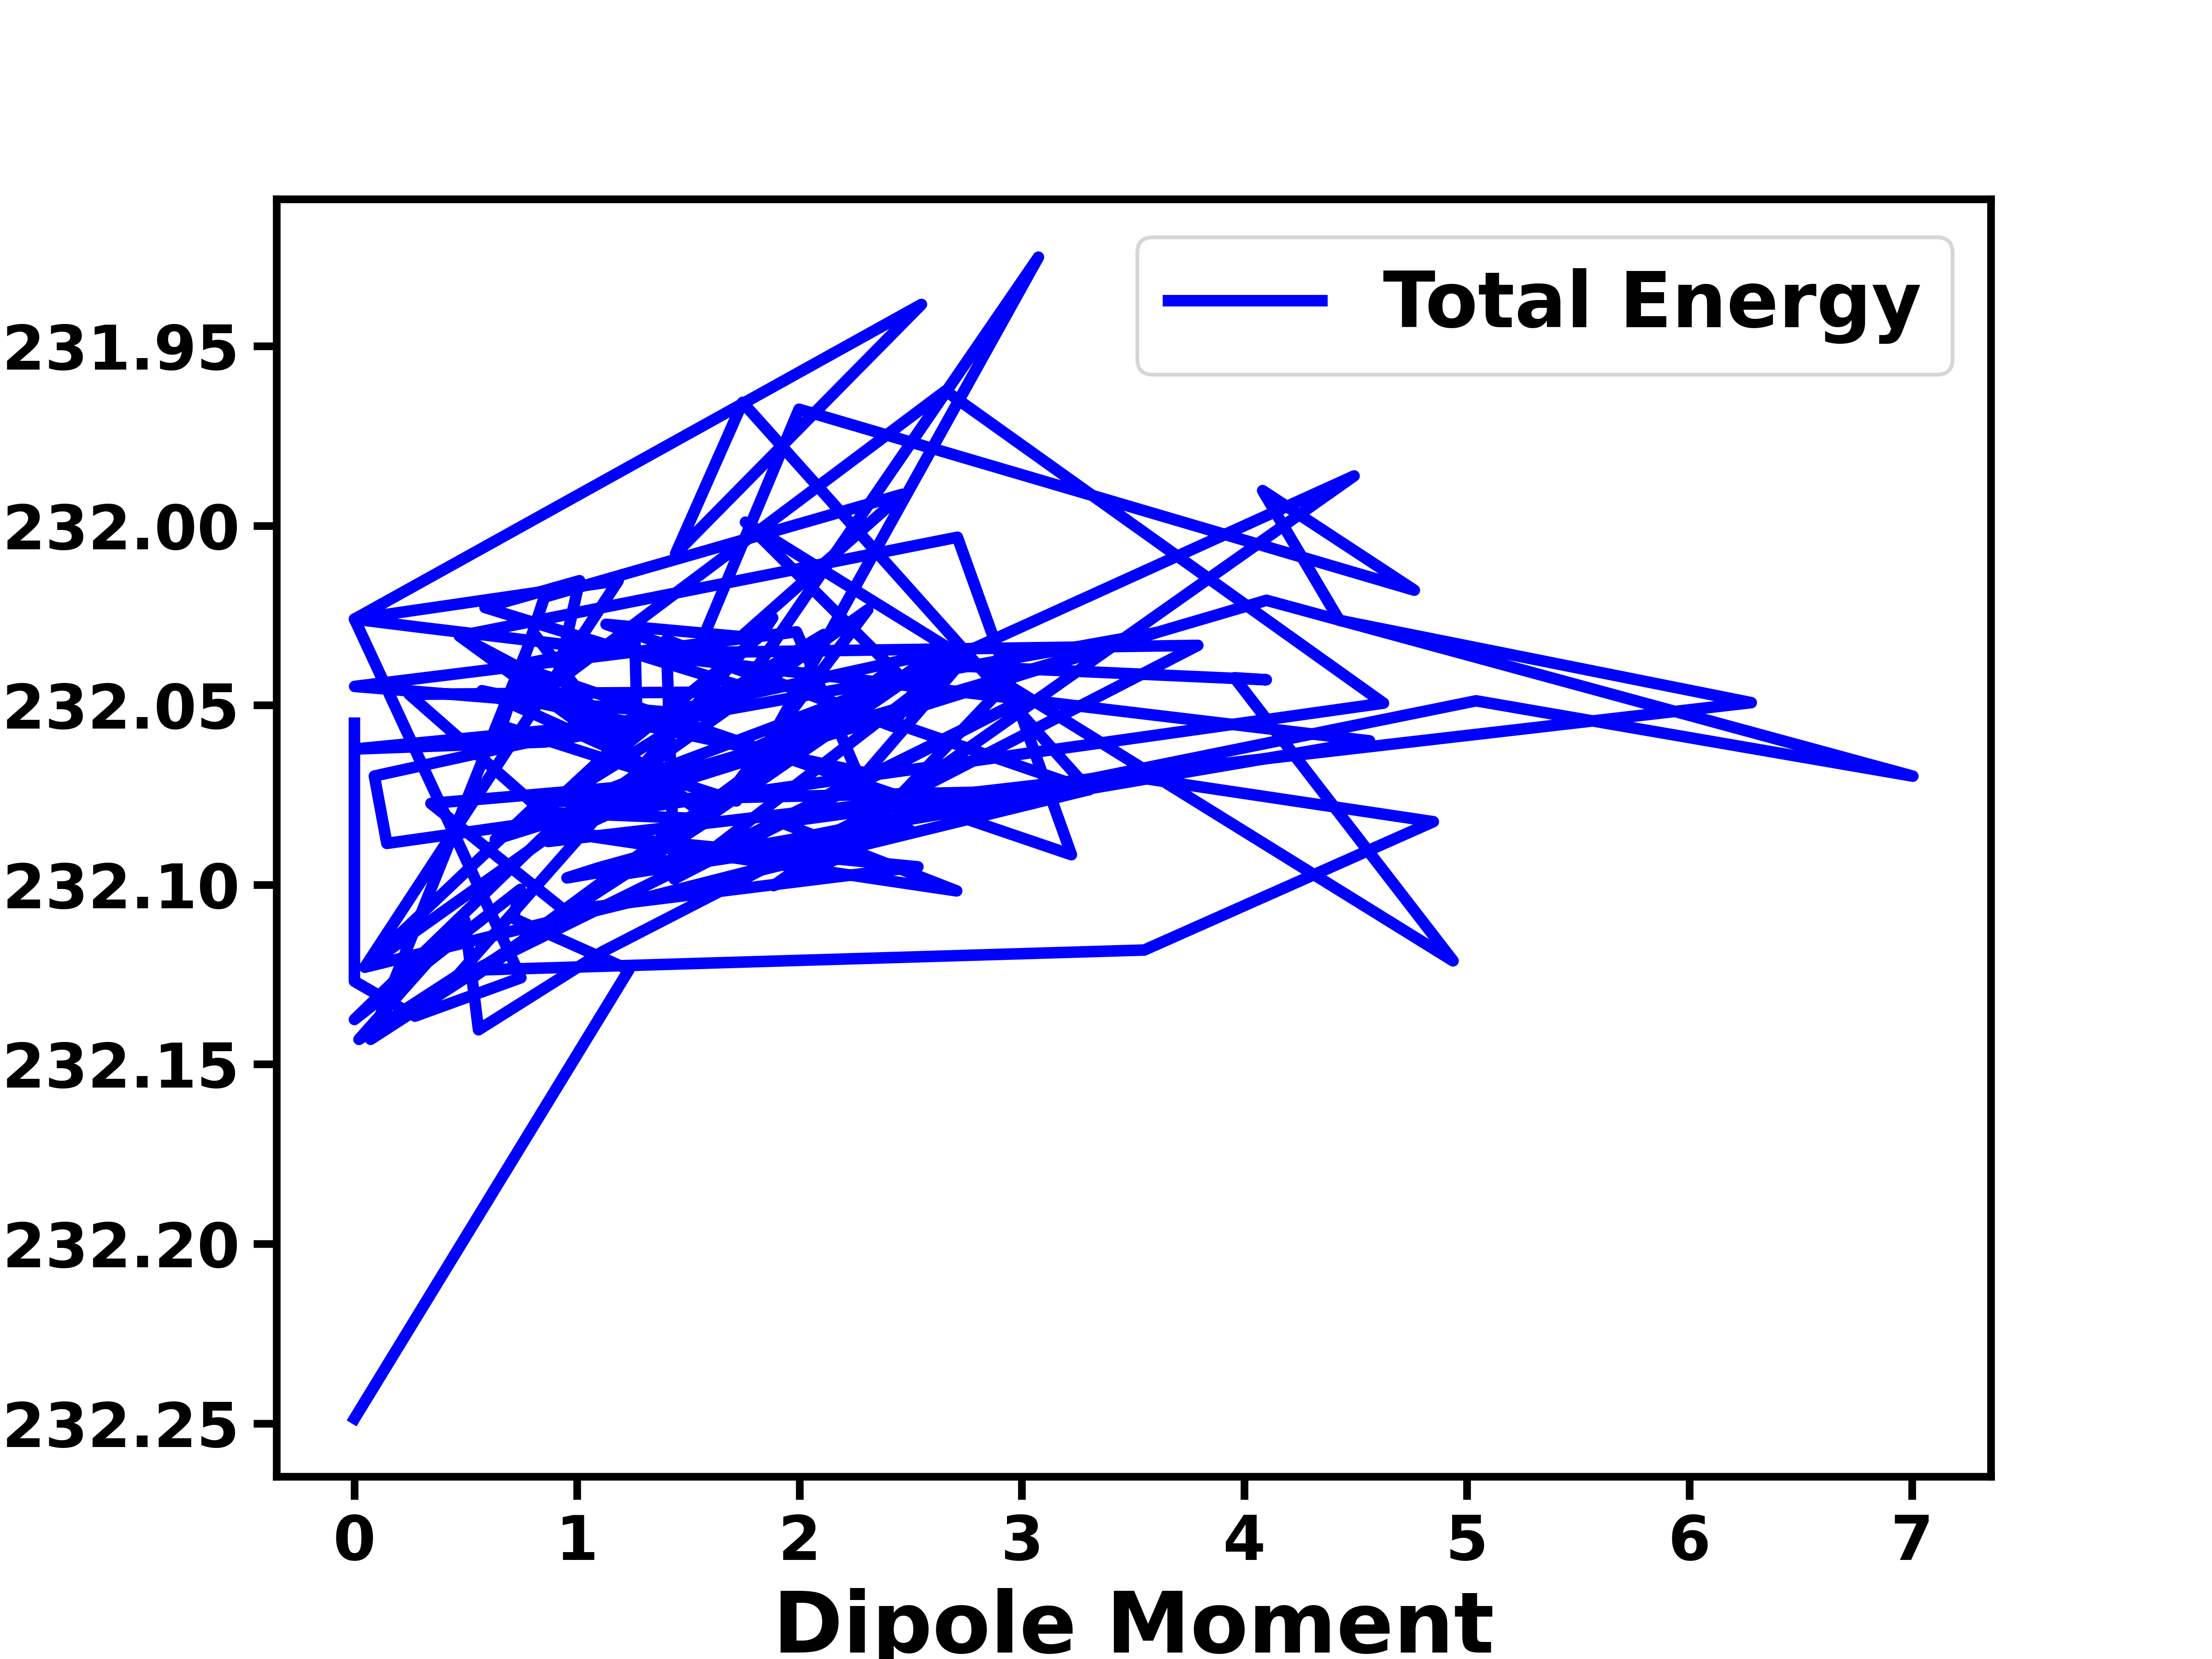
\includegraphics[scale=0.5]{Total Energy.png}
\caption{Total Energy}
\label{fig:universe}
\end{figure}

\section{Dipole Moment with HOMOE}
As we can see from the graph that the dipole moment of each isomer and the molecule's HOMOE are also not so relevant as I thought. But we can see the total energy concentrated at a certain area that ranges from 0.18 to 0.24.
\begin{figure}[H]
\centering
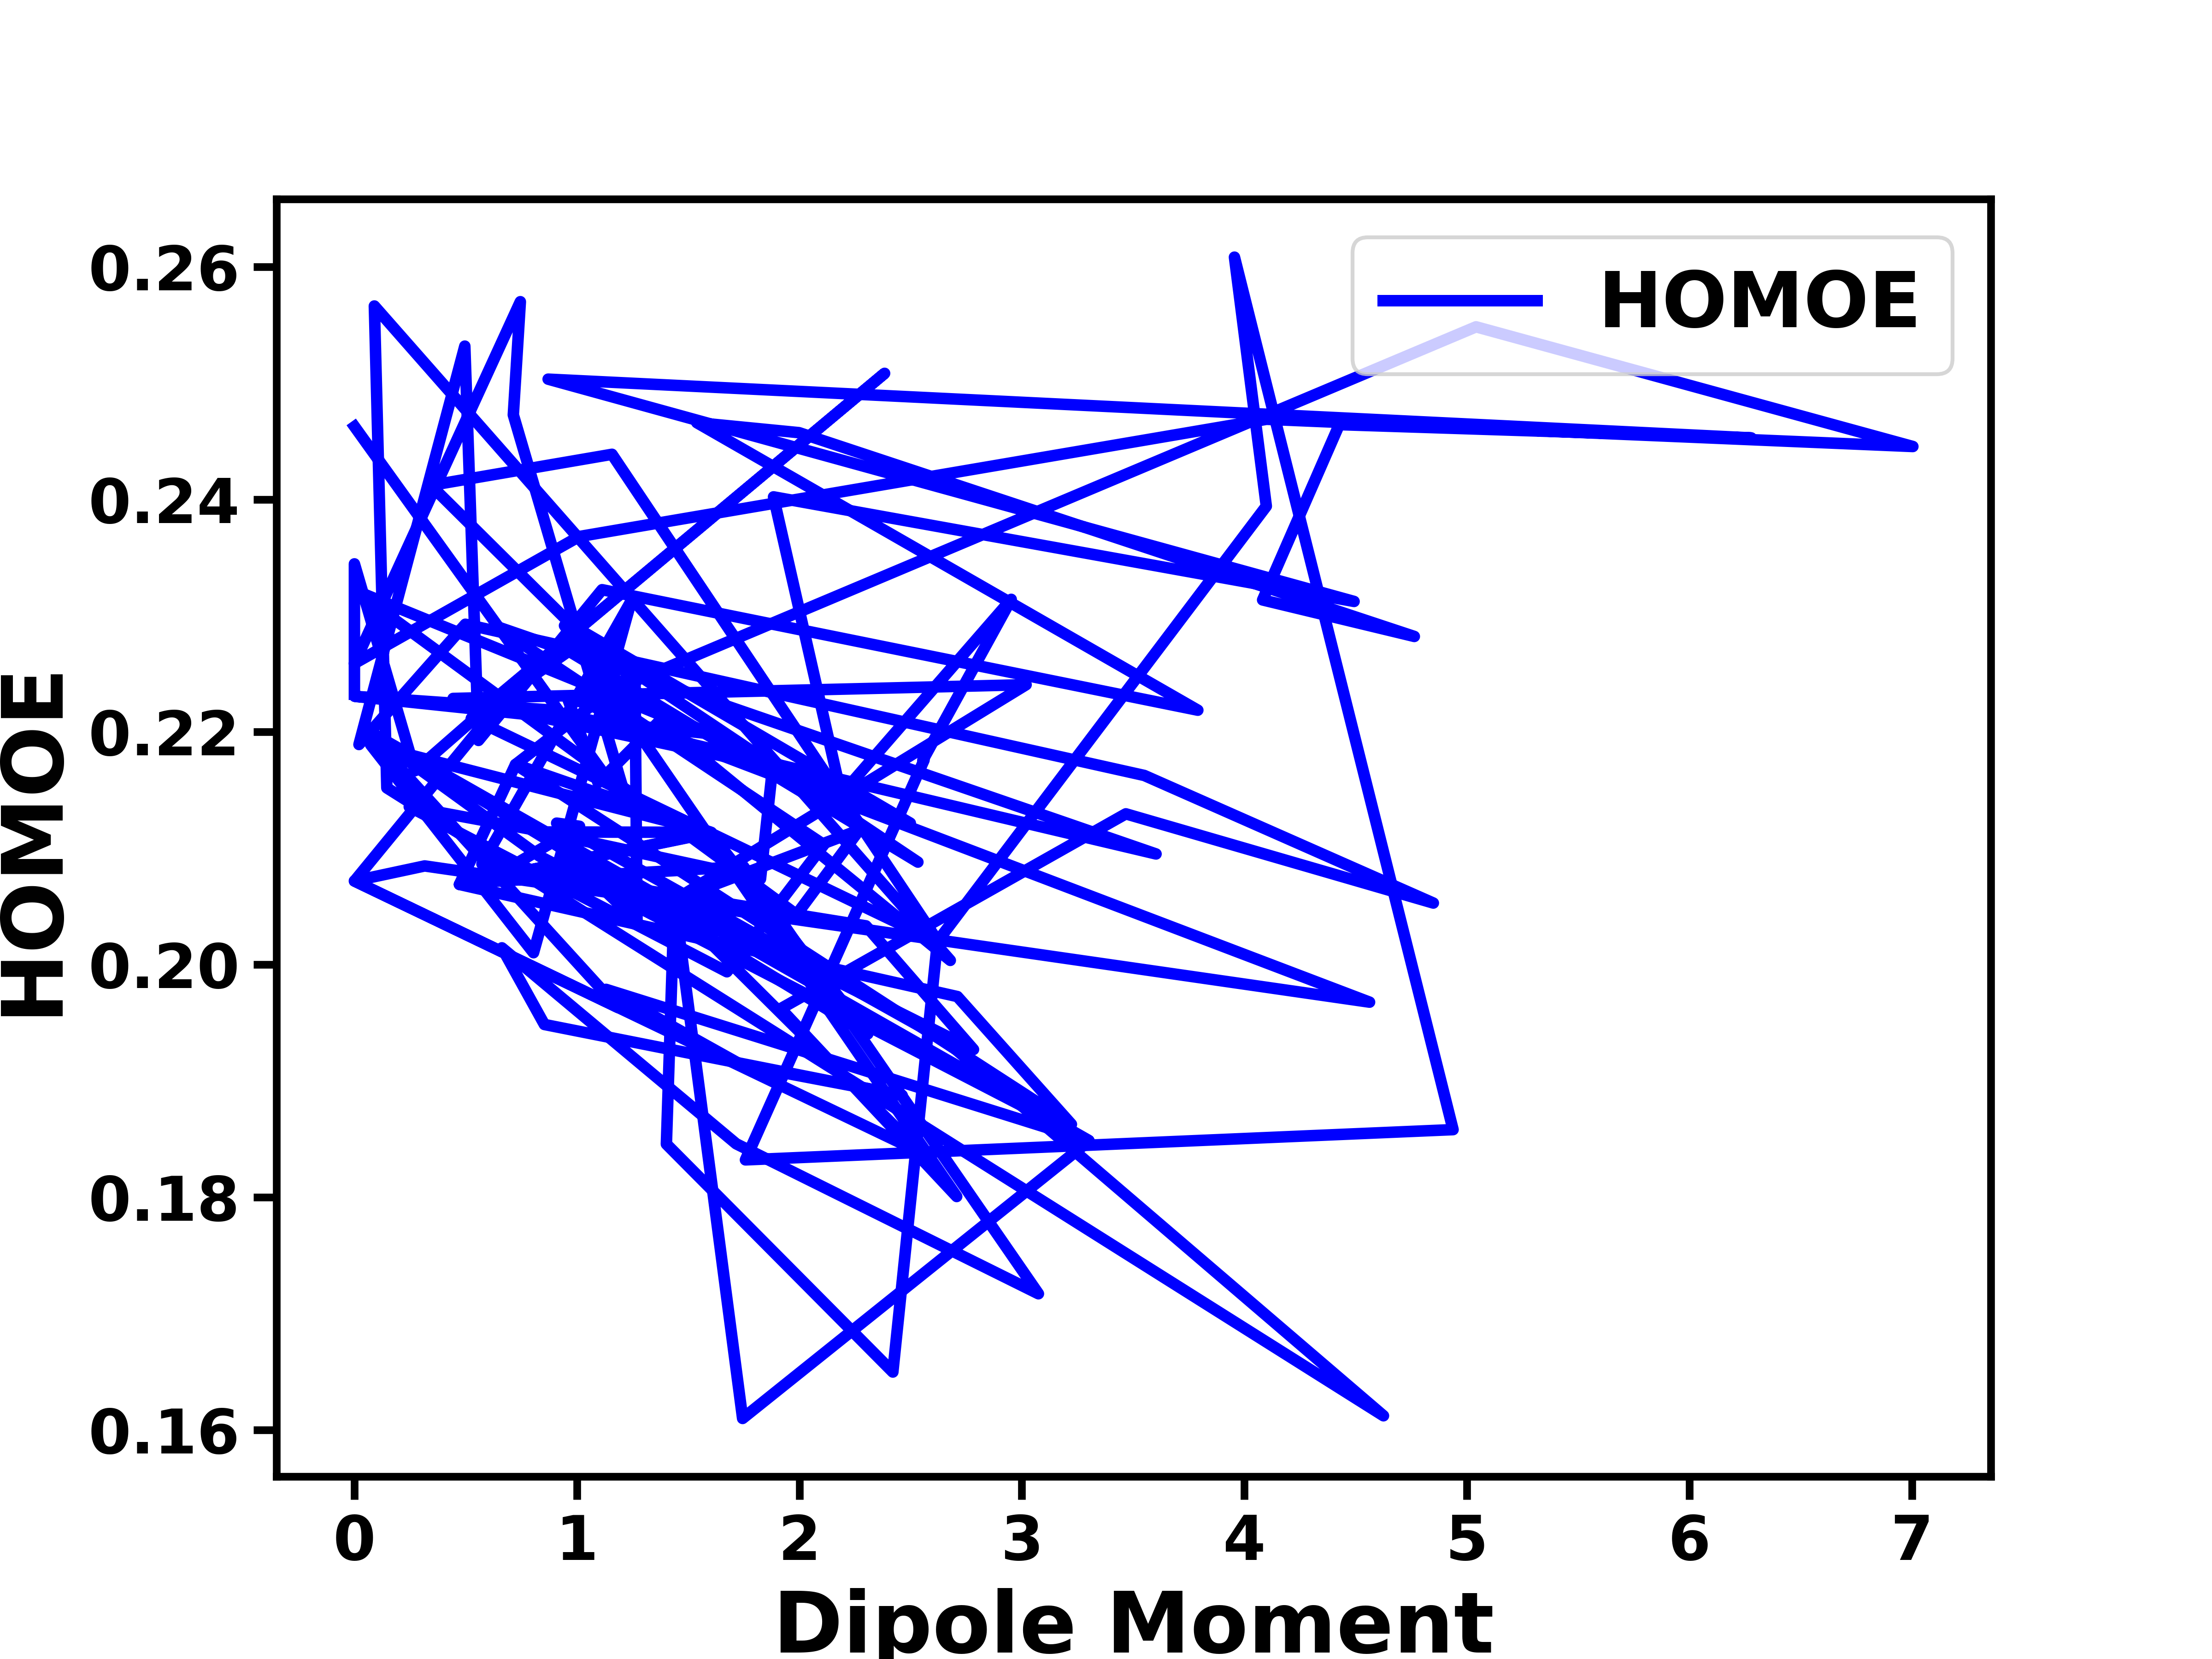
\includegraphics[scale=0.5]{HOMOE.png}
\caption{HOMOE}
\label{fig:HOMOE}
\end{figure}


\section{HOMOE with Total Energy}
As we can see from the graph that HOMOE may have a linear relationship with Total Energy, so we can import another graph to see the line's function.
\begin{figure}[H]
\centering
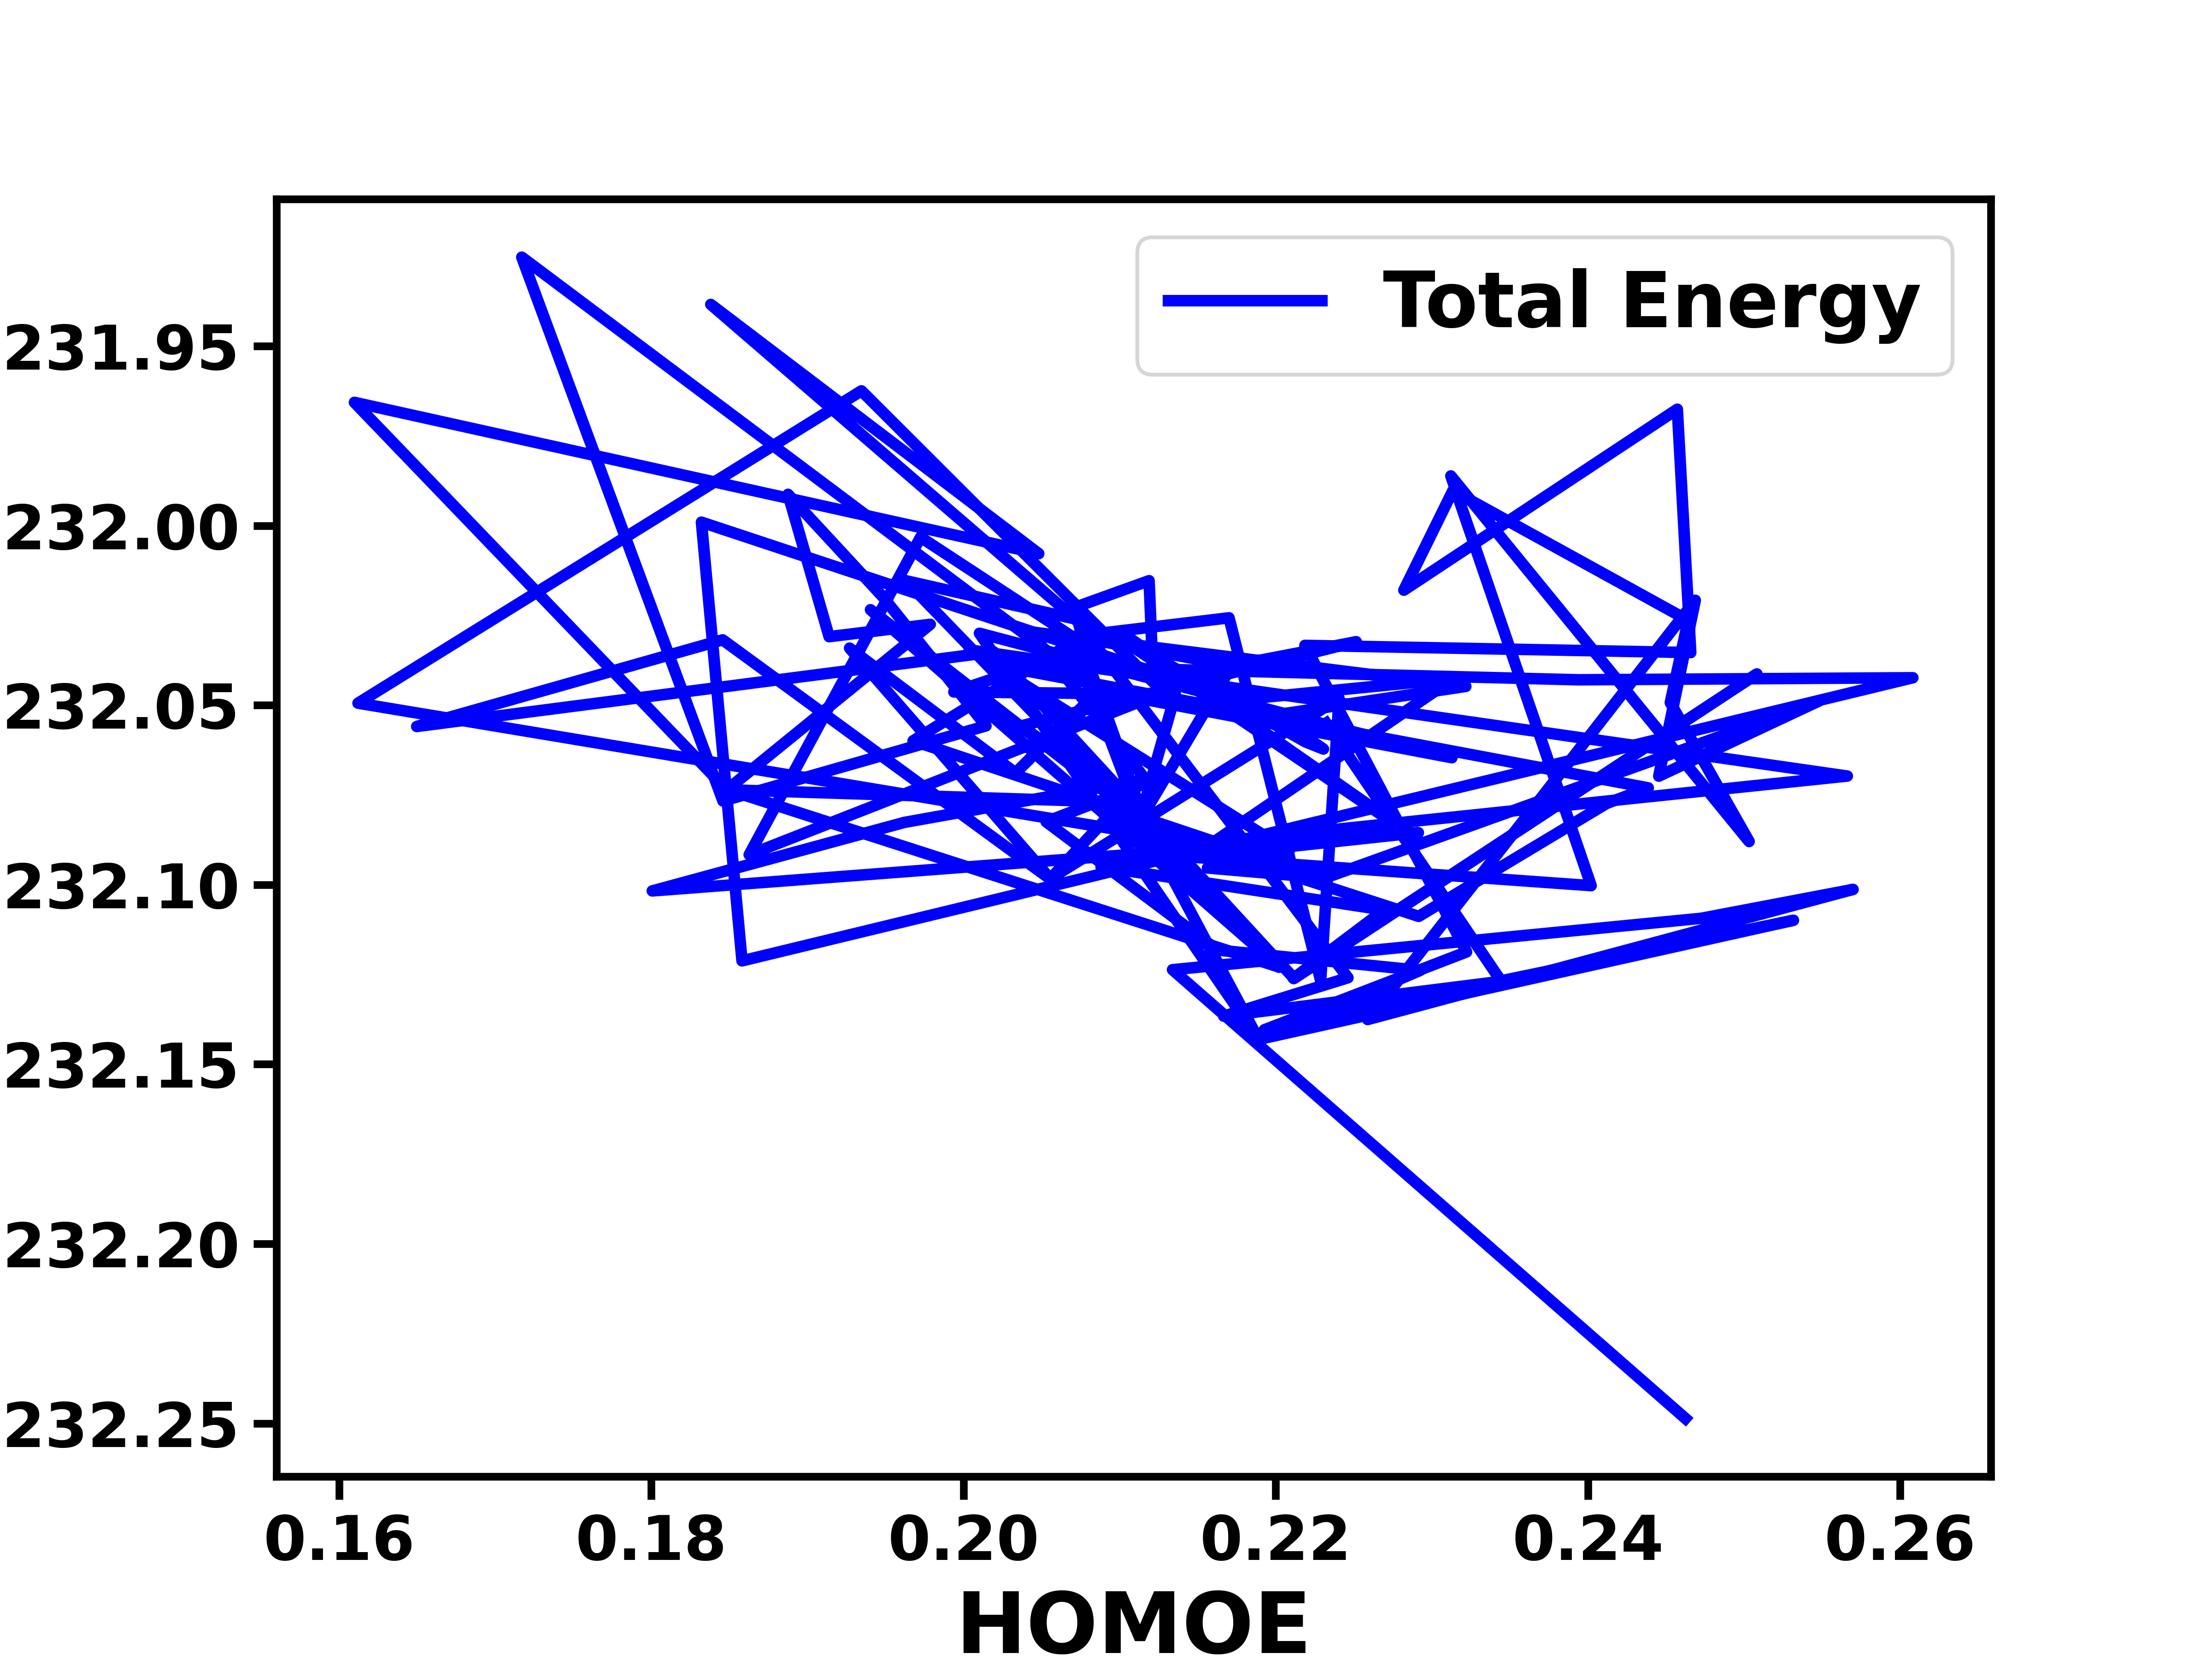
\includegraphics[scale=0.5]{Final.png}
\caption{HOMOE with Total Energy}
\label{fig:HOMOE with Total Energy}
\end{figure}
\begin{figure}[H]
\centering
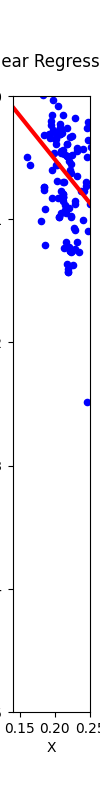
\includegraphics[scale=0.5]{lin_regression.png}
\caption{HOMOE with Total Energy(linear)}
\label{fig:HOMOE with Total Energy}
\end{figure}


\section{Conclusion}
From this experiment, I certainly did not find the relationship between dipole, total energy, and HOMOE. However, through this experiment, my understanding of quantum chemistry is deeper than before. Meanwhile, my knowledge of physics, chemistry, and computer science are expanded.


\bibliographystyle{plain}
\end{document}
